\documentclass[aspectratio=169]{beamer}

% ── Package ──
\usepackage[utf8]{inputenc}
\usepackage[T1]{fontenc}
\usepackage{graphicx}
\usepackage{booktabs}
\usepackage{listings}
\usepackage{xcolor}
\usepackage{tikz}
\usepackage{hyperref}

% ── Theme ──
\usetheme{Madrid}
\usecolortheme{whale}

% ── Warna kustom ──
\definecolor{codebg}{HTML}{F5F5F5}
\definecolor{codegreen}{HTML}{2E7D32}
\definecolor{codeorange}{HTML}{E65100}
\definecolor{codeblue}{HTML}{1565C0}

% ── Listing style ──
\lstset{
  basicstyle=\ttfamily\scriptsize,
  backgroundcolor=\color{codebg},
  keywordstyle=\color{codeblue}\bfseries,
  commentstyle=\color{codegreen},
  stringstyle=\color{codeorange},
  breaklines=true,
  frame=single,
  rulecolor=\color{gray!40},
  showstringspaces=false
}

% ── Info ──
\title[Tokorotit Testing]{Automated UI Testing\\Aplikasi Tokorotit}
\subtitle{Menggunakan Cucumber BDD + Selenium WebDriver}
\author{Tim QA}
\institute{}
\date{\today}

% ══════════════════════════════════════════════════════════════
%  SLIDE 1 — COVER
% ══════════════════════════════════════════════════════════════
\begin{document}

\begin{frame}
  \titlepage
\end{frame}

% ══════════════════════════════════════════════════════════════
%  SLIDE 2 — DAFTAR ISI
% ══════════════════════════════════════════════════════════════
\begin{frame}{Daftar Isi}
  \tableofcontents
\end{frame}

% ══════════════════════════════════════════════════════════════
%  SECTION 1 — PENDAHULUAN
% ══════════════════════════════════════════════════════════════
\section{Pendahuluan}

% ── SLIDE 3 — Latar Belakang ──
\begin{frame}{Latar Belakang}
  \begin{itemize}
    \item Pengujian manual memakan waktu dan rentan human error
    \item Aplikasi \textbf{Tokorotit} memiliki banyak fitur CRUD yang perlu diuji secara konsisten
    \item Dibutuhkan \textbf{automated UI testing} untuk menjamin kualitas aplikasi secara berkelanjutan
    \item Pendekatan \textbf{BDD (Behavior-Driven Development)} dipilih agar skenario test mudah dibaca oleh semua stakeholder
  \end{itemize}
\end{frame}

% ── SLIDE 4 — Tujuan ──
\begin{frame}{Tujuan Pengujian}
  \begin{enumerate}
    \item Memverifikasi fungsionalitas \textbf{login} untuk peran Admin dan Branch
    \item Menguji operasi \textbf{CRUD} pada master data (User, Product, Expense, Branch)
    \item Memvalidasi \textbf{input validation} — memastikan pesan error muncul saat form kosong
    \item Menguji fitur cabang: \textbf{Branch Product, Product History, Expense History}
    \item Memastikan aplikasi berjalan sesuai spesifikasi secara \textbf{otomatis dan repeatable}
  \end{enumerate}
\end{frame}

% ══════════════════════════════════════════════════════════════
%  SECTION 2 — SYSTEM UNDER TEST (SUT)
% ══════════════════════════════════════════════════════════════
\section{System Under Test (SUT)}

% ── SLIDE 5 — Deskripsi SUT ──
\begin{frame}{Deskripsi Aplikasi Tokorotit}
  \textbf{Tokorotit} adalah aplikasi web manajemen toko/cabang yang berjalan di:
  \begin{center}
    \texttt{http://127.0.0.1:8000}
  \end{center}

  \vspace{0.5em}
  \textbf{Dua peran pengguna:}
  \begin{table}[h]
    \centering
    \begin{tabular}{llll}
      \toprule
      \textbf{Peran} & \textbf{Username} & \textbf{Dashboard} & \textbf{Akses Utama} \\
      \midrule
      Admin   & \texttt{admin}    & \texttt{/admin}  & Kelola master data \\
      Branch  & \texttt{employee} & \texttt{/branch} & Kelola data cabang \\
      \bottomrule
    \end{tabular}
  \end{table}
\end{frame}

% ── SLIDE 6 — Halaman yang Diuji ──
\begin{frame}{Halaman-halaman yang Diuji}
  \begin{columns}[T]
    \begin{column}{0.48\textwidth}
      \textbf{Sisi Admin:}
      \begin{itemize}
        \item \texttt{/login} — Login
        \item \texttt{/admin} — Dashboard
        \item \texttt{/admin/users} — Master User
        \item \texttt{/admin/products} — Master Product
        \item \texttt{/admin/expenses} — Master Expense
        \item \texttt{/admin/branches} — Master Branch
      \end{itemize}
    \end{column}
    \begin{column}{0.48\textwidth}
      \textbf{Sisi Branch:}
      \begin{itemize}
        \item \texttt{/branch} — Dashboard
        \item \texttt{/branch/products} — Branch Products
        \item \texttt{/branch/history/products} — Product History
        \item \texttt{/branch/history/expenses} — Expense History
      \end{itemize}
    \end{column}
  \end{columns}
\end{frame}

% ══════════════════════════════════════════════════════════════
%  SECTION 3 — TECH STACK
% ══════════════════════════════════════════════════════════════
\section{Tech Stack}

% ── SLIDE 7 — Teknologi yang Digunakan ──
\begin{frame}{Teknologi yang Digunakan}
  \begin{table}[h]
    \centering
    \begin{tabular}{lll}
      \toprule
      \textbf{Komponen} & \textbf{Teknologi} & \textbf{Versi} \\
      \midrule
      Bahasa Pemrograman & Java               & 21      \\
      Build Tool         & Maven              & —       \\
      BDD Framework      & Cucumber           & 7.20.1  \\
      Test Runner        & JUnit 5 (Platform Suite) & 5.11.3 \\
      Browser Automation & Selenium WebDriver & 4.44.0  \\
      Browser            & Microsoft Edge     & —       \\
      DI Container       & Cucumber PicoContainer & —   \\
      \bottomrule
    \end{tabular}
  \end{table}
\end{frame}

% ── SLIDE 8 — Mengapa Cucumber + Selenium? ──
\begin{frame}{Mengapa Cucumber + Selenium?}
  \begin{columns}[T]
    \begin{column}{0.48\textwidth}
      \textbf{Cucumber (BDD):}
      \begin{itemize}
        \item Skenario ditulis dalam bahasa natural (Gherkin)
        \item Mudah dipahami oleh non-developer
        \item Format \texttt{Given-When-Then} yang terstruktur
        \item Menjembatani komunikasi antara tim bisnis dan teknis
      \end{itemize}
    \end{column}
    \begin{column}{0.48\textwidth}
      \textbf{Selenium WebDriver:}
      \begin{itemize}
        \item Otomasi browser secara langsung
        \item Support multi-browser (Edge, Chrome, Firefox)
        \item Interaksi realistis seperti pengguna asli
        \item Komunitas besar dan dokumentasi lengkap
      \end{itemize}
    \end{column}
  \end{columns}
\end{frame}

% ══════════════════════════════════════════════════════════════
%  SECTION 4 — ARSITEKTUR TEST
% ══════════════════════════════════════════════════════════════
\section{Arsitektur Test}

% ── SLIDE 9 — Struktur Proyek ──
\begin{frame}[fragile]{Struktur Proyek}
\begin{lstlisting}[language={},title={Struktur Direktori}]
src/test/
  java/
    runner/
      TestRunner.java          <- Cucumber runner
    stepDefinitions/
      Hooks.java               <- Setup & teardown browser
      LoginPage.java           <- Page Object: Login
      AdminMasterUserPage.java <- Page Object: Master User
      ...                      <- Page Object lainnya
      LoginSteps.java          <- Step Definitions: Login
      MasterUserSteps.java     <- Step Definitions: User
      ...                      <- Step Definitions lainnya
  resources/
    features/
      login.feature            <- Gherkin: Login
      masteruser.feature       <- Gherkin: Master User
      ...                      <- Feature file lainnya
\end{lstlisting}
\end{frame}

% ── SLIDE 10 — Pola Desain: Page Object Model ──
\begin{frame}{Pola Desain: Page Object Model (POM)}
  \begin{center}
    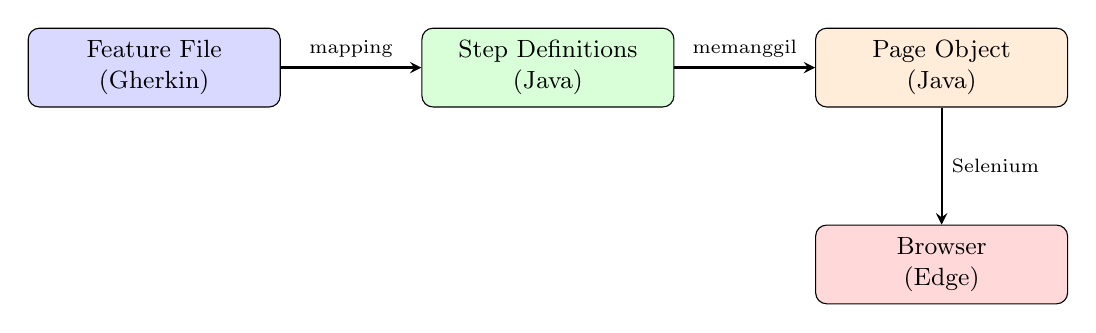
\begin{tikzpicture}[
      box/.style={rectangle, draw, rounded corners, minimum width=3.2cm, minimum height=1cm, align=center, font=\small},
      arrow/.style={->, thick, >=stealth}
    ]
      \node[box, fill=blue!15]   (feature) at (0,0)    {Feature File\\(Gherkin)};
      \node[box, fill=green!15]  (steps)   at (5,0)    {Step Definitions\\(Java)};
      \node[box, fill=orange!15] (page)    at (10,0)   {Page Object\\(Java)};
      \node[box, fill=red!15]    (browser) at (10,-2.5){Browser\\(Edge)};

      \draw[arrow] (feature) -- (steps) node[midway, above] {\scriptsize mapping};
      \draw[arrow] (steps)   -- (page)  node[midway, above] {\scriptsize memanggil};
      \draw[arrow] (page)    -- (browser) node[midway, right] {\scriptsize Selenium};
    \end{tikzpicture}
  \end{center}

  \vspace{0.5em}
  \begin{itemize}
    \item \textbf{Feature File} → mendefinisikan skenario dalam bahasa Gherkin
    \item \textbf{Step Definitions} → menghubungkan langkah Gherkin ke kode Java
    \item \textbf{Page Object} → mengenkapsulasi elemen UI dan interaksi per halaman
  \end{itemize}
\end{frame}

% ── SLIDE 11 — Hooks: Setup \& Teardown ──
\begin{frame}[fragile]{Hooks: Setup \& Teardown}
  Setiap scenario dijalankan dengan siklus:

\begin{lstlisting}[language=Java, title={Hooks.java (disederhanakan)}]
public class Hooks {
    public static WebDriver driver;
    public static LoginPage loginPage;
    // ... page object lainnya

    @Before
    public void setupDriver() {
        driver = new EdgeDriver();
        loginPage = new LoginPage(driver);
        // inisialisasi semua page object
        driver.manage().timeouts()
              .implicitlyWait(Duration.ofSeconds(3));
        driver.manage().window().maximize();
    }

    @After
    public void closeBrowser() {
        driver.quit();
    }
}
\end{lstlisting}
\end{frame}

% ══════════════════════════════════════════════════════════════
%  SECTION 5 — TEST SCENARIO
% ══════════════════════════════════════════════════════════════
\section{Test Scenario}

% ── SLIDE 12 — Ringkasan Scenario ──
\begin{frame}{Ringkasan Test Scenario}
  Total: \textbf{8 feature file} dengan \textbf{13 scenario}

  \begin{table}[h]
    \centering\small
    \begin{tabular}{llcc}
      \toprule
      \textbf{Feature} & \textbf{Peran} & \textbf{Valid} & \textbf{Invalid} \\
      \midrule
      Login            & Admin/Branch & 2 & 1 \\
      Master User      & Admin        & 1 & 1 \\
      Master Product   & Admin        & 1 & 1 \\
      Master Expense   & Admin        & 1 & 1 \\
      Master Branch    & Admin        & 1 & 1 \\
      Branch Product   & Branch       & — & 1 \\
      Product History  & Branch       & — & 1 \\
      Expense History  & Branch       & — & 1 \\
      \midrule
      \textbf{Total}   &              & \textbf{6} & \textbf{7} \\
      \bottomrule
    \end{tabular}
  \end{table}
\end{frame}

% ── SLIDE 13 — Scenario: Login ──
\begin{frame}[fragile]{Scenario: Login (3 Skenario)}
\begin{lstlisting}[language={},title={login.feature}]
Feature: User Login

Background:
  Given User is in login page

Scenario: Successful admin login
  When Write valid admin username and password
       then presses the submit button
  Then Arrive at admin dashboard

Scenario: Successful branch login
  When Write valid branch account username and password
       then presses the submit button
  Then Arrive at branch dashboard

Scenario: Invalid credentials
  When Write invalid username and password
       then presses the submit button
  Then Stays at login page
\end{lstlisting}
\end{frame}

% ── SLIDE 14 — Scenario: Master User ──
\begin{frame}[fragile]{Scenario: Master User (2 Skenario)}
\begin{lstlisting}[language={},title={masteruser.feature}]
Feature: Master User

Background:
  Given User is logged in as admin
        then opens users CRUD page

Scenario: Add new user valid
  When Press New User then enter valid user data
       then submit
  Then Get "User created successfully" message

Scenario: Add new user invalid
  When Press New User then press submit
       with fields empty
  Then Get "Please fill required fields.
       Password required for new user." message
\end{lstlisting}

  \vspace{0.3em}
  \small\textit{Pola yang sama diterapkan untuk Master Product, Expense, dan Branch.}
\end{frame}

% ── SLIDE 15 — Scenario: Master Product, Expense, Branch ──
\begin{frame}{Scenario: Master Product, Expense, Branch}
  Ketiga modul mengikuti pola test yang sama:

  \begin{table}[h]
    \centering\small
    \begin{tabular}{lll}
      \toprule
      \textbf{Feature} & \textbf{Valid Case (Pesan Sukses)} & \textbf{Invalid Case (Pesan Error)} \\
      \midrule
      Master Product & ``Product created successfully.'' & ``Please enter name and price'' \\
      Master Expense & ``Expense created successfully.'' & ``Please enter an expense name'' \\
      Master Branch  & ``Branch created successfully.''  & ``Please enter a branch name'' \\
      \bottomrule
    \end{tabular}
  \end{table}

  \vspace{0.5em}
  \textbf{Alur test:}
  \begin{enumerate}
    \item Login sebagai admin → navigasi ke halaman CRUD
    \item \textit{Valid}: isi form dengan data → submit → verifikasi pesan sukses
    \item \textit{Invalid}: langsung submit form kosong → verifikasi pesan error
  \end{enumerate}
\end{frame}

% ── SLIDE 16 — Scenario: Fitur Branch ──
\begin{frame}{Scenario: Fitur Branch (3 Skenario)}
  Test untuk sisi \textbf{Branch user} (login sebagai \texttt{employee}):

  \begin{table}[h]
    \centering\small
    \begin{tabular}{ll}
      \toprule
      \textbf{Feature} & \textbf{Invalid Case (Pesan Error)} \\
      \midrule
      Branch Product   & ``Please select a product and enter branch price'' \\
      Product History  & ``Please fill all required fields'' \\
      Expense History  & ``Please fill all required fields'' \\
      \bottomrule
    \end{tabular}
  \end{table}

  \vspace{0.5em}
  \textbf{Alur test:}
  \begin{enumerate}
    \item Login sebagai branch user (\texttt{employee / employee123})
    \item Navigasi ke halaman terkait
    \item Tekan tombol Add → langsung submit tanpa mengisi field
    \item Verifikasi pesan error validasi muncul
  \end{enumerate}
\end{frame}

% ══════════════════════════════════════════════════════════════
%  SECTION 6 — CONTOH KODE
% ══════════════════════════════════════════════════════════════
\section{Contoh Implementasi}

% ── SLIDE 17 — Page Object: LoginPage ──
\begin{frame}[fragile]{Page Object: LoginPage.java}
\begin{lstlisting}[language=Java]
public class LoginPage {
    private WebDriver driver;
    private By usernamefield = new By.ById("username");
    private By passwordfield = new By.ById("password");
    private By submitbutton  = new By.ByXPath(
        "/html/body/div[1]/div/form/button");

    public LoginPage(WebDriver d) {
        this.driver = d;
    }

    public void setUsername(String s) {
        driver.findElement(usernamefield).sendKeys(s);
    }
    public void setPassword(String s) {
        driver.findElement(passwordfield).sendKeys(s);
    }
    public void submit() {
        driver.findElement(submitbutton).click();
    }
}
\end{lstlisting}
\end{frame}

% ── SLIDE 18 — Step Definition: LoginSteps ──
\begin{frame}[fragile]{Step Definition: LoginSteps.java}
\begin{lstlisting}[language=Java]
public class LoginSteps {

    @Given("User is in login page")
    public void userinloginpage() {
        Hooks.driver.get("http://127.0.0.1:8000/login");
    }

    @When("Write valid admin username and password ...")
    public void admincredential() {
        Hooks.loginPage.setUsername("admin");
        Hooks.loginPage.setPassword("admin123");
        Hooks.loginPage.submit();
    }

    @Then("Arrive at admin dashboard")
    public void arriveadmin() {
        String expectedURL = "http://127.0.0.1:8000/admin";
        WebDriverWait wait = new WebDriverWait(
            Hooks.driver, Duration.ofSeconds(10));
        // verifikasi URL sesuai ekspektasi
        Assertions.assertEquals(
            Hooks.driver.getCurrentUrl(), expectedURL);
    }
}
\end{lstlisting}
\end{frame}

% ══════════════════════════════════════════════════════════════
%  SECTION 7 — CARA MENJALANKAN
% ══════════════════════════════════════════════════════════════
\section{Cara Menjalankan}

% ── SLIDE 19 — Prasyarat \& Eksekusi ──
\begin{frame}[fragile]{Cara Menjalankan Test}
  \textbf{Prasyarat:}
  \begin{itemize}
    \item Java 21+ terinstal
    \item Maven terinstal
    \item Microsoft Edge browser terinstal
    \item Aplikasi Tokorotit berjalan di \texttt{http://127.0.0.1:8000}
  \end{itemize}

  \vspace{1em}
  \textbf{Eksekusi:}
\begin{lstlisting}[language=bash]
# Jalankan semua test
mvn test

# Jalankan feature tertentu (contoh: login saja)
mvn test -Dcucumber.features="src/test/resources/features/login.feature"
\end{lstlisting}

  \vspace{0.5em}
  Test runner akan:
  \begin{enumerate}
    \item Membuka browser Edge secara otomatis
    \item Menjalankan setiap scenario satu per satu
    \item Menutup browser setelah setiap scenario selesai
    \item Menampilkan hasil pass/fail di console
  \end{enumerate}
\end{frame}

% ══════════════════════════════════════════════════════════════
%  SECTION 8 — KESIMPULAN
% ══════════════════════════════════════════════════════════════
\section{Kesimpulan}

% ── SLIDE 20 — Kesimpulan ──
\begin{frame}{Kesimpulan}
  \begin{itemize}
    \item Berhasil membuat \textbf{13 automated test scenario} yang mencakup fungsionalitas utama aplikasi Tokorotit
    \item Menggunakan pendekatan \textbf{BDD (Cucumber)} sehingga skenario mudah dipahami
    \item Menerapkan \textbf{Page Object Model} untuk kode test yang terstruktur dan mudah di-maintain
    \item Test mencakup \textbf{positive case} (input valid) dan \textbf{negative case} (validasi input kosong)
    \item Test dapat dijalankan secara \textbf{otomatis dan berulang} dengan satu perintah \texttt{mvn test}
  \end{itemize}

  \vspace{1em}
  \begin{block}{Pengembangan Selanjutnya}
    \begin{itemize}
      \item Menambahkan test untuk operasi \textbf{Update} dan \textbf{Delete}
      \item Menambahkan \textbf{valid case} untuk fitur Branch (product, history)
      \item Integrasi dengan \textbf{CI/CD pipeline} untuk pengujian otomatis
      \item Menambahkan \textbf{test report} (Cucumber HTML Report / Allure)
    \end{itemize}
  \end{block}
\end{frame}

% ══════════════════════════════════════════════════════════════
%  SLIDE 21 — TERIMA KASIH
% ══════════════════════════════════════════════════════════════
\begin{frame}
  \centering
  \Huge\bfseries Terima Kasih

  \vspace{1em}
  \Large Sesi Tanya Jawab
\end{frame}

\end{document}
